\section{Installing and Starting}

\subsection{Desktop Application}

The desktop application requires the Java Runtime Environment (JRE) available
from \url{http://www.java.com/en/download/index.jsp}. The application has been
tested on JRE 6 and JRE 7 without issue. The print functionality
requires a pre-installed \LaTeX distribution that includes the
executable `pdflatex'. The installation procedure varies for each
operating system and instructions are available from:
\url{http://latex-project.org/ftp.html}.

After the Java Runtime Environment (JRE) is installed, running the application
can be achieved by executing the following command from any terminal
window:
\begin{verbatim}
java -jar TeamW-SportsElim.jar
\end{verbatim}
or by launching from your favourite file browser.

A \LaTeX distrabution is not required to run the core of the
application, only the print functionality. In the event that the
command `pdflatex' cannot be found, the application will fail to print
however will not crash. Print functionality is known to work on
standard installations of the distribution on Linux/GNU-based and Mac
OS operating system. 

\subsection{Web Application}

Installation of the web application is not required as a remote host is running
the required software. This can be accessed via
\url{http://www.gordonrenfrewshire.com/teamw}. For purposes of completeness and
satisfying the potential desires of the reader, an installation procedure was
supplied in Appendix~\ref{sec:install}.

In the event that the supplied URL fails to work, please contact Gordon Reid via
any of the following methods:

Student email: 1002536r@student.gla.ac.uk

Personal email: gordon.reid1992@hotmail.co.uk

Mobile phone: 07706 477 672

\section{Desktop Navigation}

\begin{figure}
  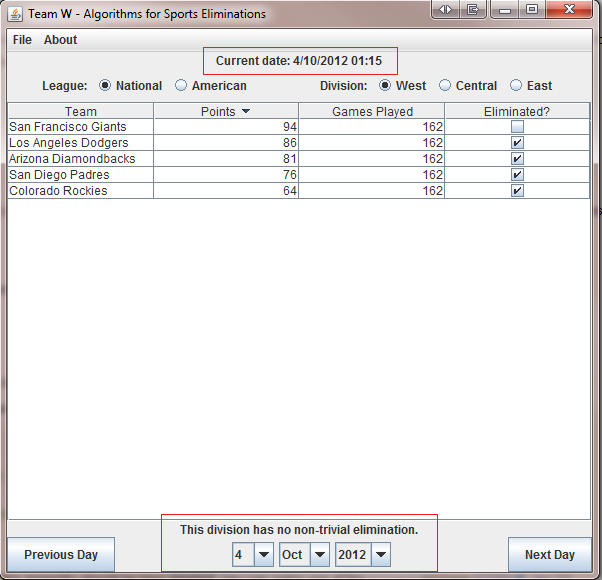
\includegraphics[width=\linewidth,keepaspectratio]{images/userManualDesk1.png}
  \caption{Starting Screen}\label{fig:STARTSCREEN}
\end{figure}
Upon launching, you will see the screen in Figure~\ref{fig:STARTSCREEN}.
Highlighted in the red box at the bottom of the screen is the
main navigational tool for traversing to different dates within the
season. Three dropdown selectors allow you to instantly jump to any
date in the season. Simple day-by-day navigation can be achieved
using the buttons in the bottom left and bottom right of
Figure~\ref{fig:STARTSCREEN} and these allow you to navigate backwards
or forwards in the league respectively.
The application will always start at the last date in the season it
knows about. The current date and time relating to the information on
screen is displayed in the red box at the top of the screen.

\begin{figure}
  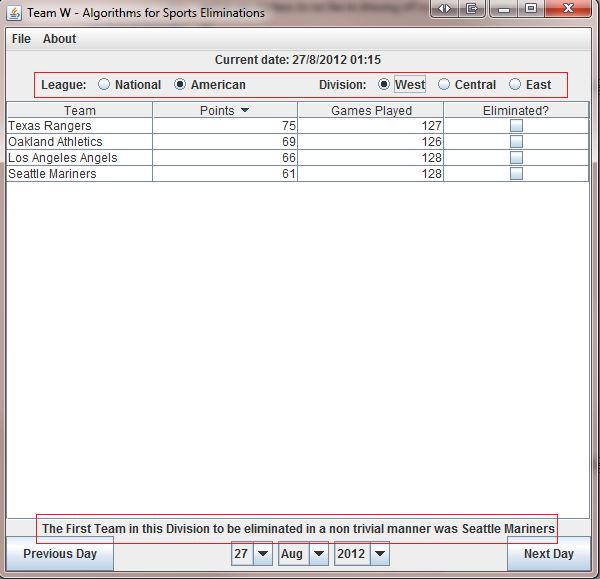
\includegraphics[width=\linewidth,keepaspectratio]{images/userManualDesk3.png}
  \caption{League Navigation}\label{fig:LEAGNAV}
\end{figure}
The radio buttons highlighted at the top of Figure~\ref{fig:LEAGNAV}
allow you to change between the various divisions supported by the
application. There are a total of six combinations. The date you
are currently on transfers when you change league, for example if you
are viewing the ``National West'' division on ``27/8/2012 01:15'' and
you change to ``Nationa East'' you will see the results of the
``National East'' division on ``27/8/2012 01:15''. The first
non-trivial elimination information for the currently selected
division is shown in the highlighted red box at the bottom of
Figure~\ref{fig:LEAGNAV}

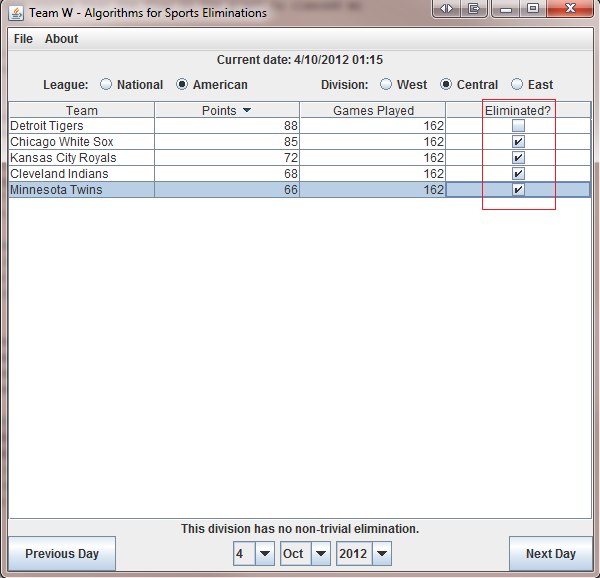
\includegraphics[width=\linewidth,keepaspectratio]{images/userManualDesk4.png}

If you click on one of the checked boxes available specifying that a team has
been eliminated, it will you show the certificate of elimination - which team
was responsible for it's elimination, or if it wasn't a team, the fact that
they're not top when the season has finished as shown below.

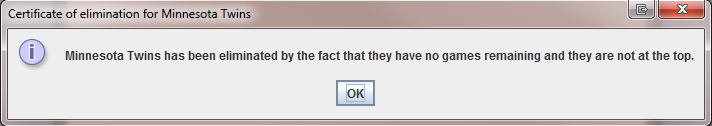
\includegraphics[width=\linewidth,keepaspectratio]{images/userManualDesk5.png}

If we change the date and league and click on a team this time we're able to see
the elimination as consequence of another team.

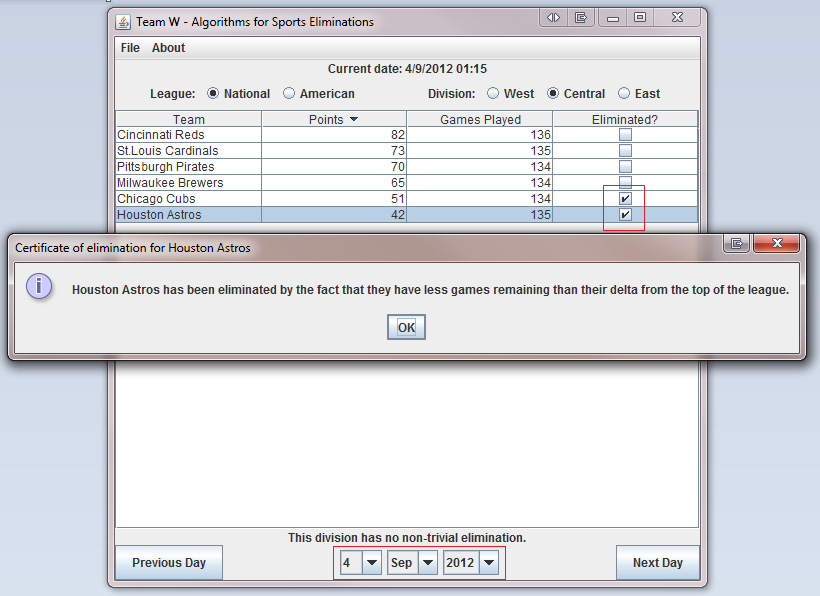
\includegraphics[width=\linewidth,keepaspectratio]{images/userManualDesk6.png}

\newpage

\section{Importing}

The import functionality within the program allows user specified seasons to be
used in the system directly if they wish to analyse future or prior seasons,
they need only follow the formatting conventions used in the original source and
when they're prompted to select a file they select a suitable file the
application will calculate and generate the appropriate results up to whatever
date the users file goes up to.

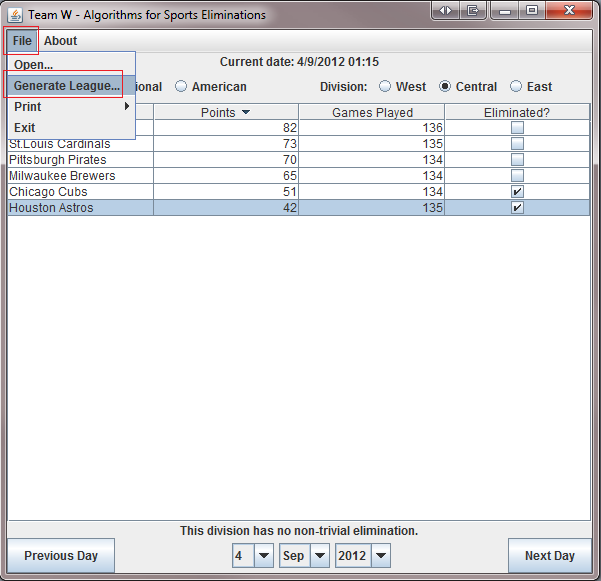
\includegraphics[width=\linewidth,height=\measurepage,keepaspectratio]
{images/userManualDesk7.png}

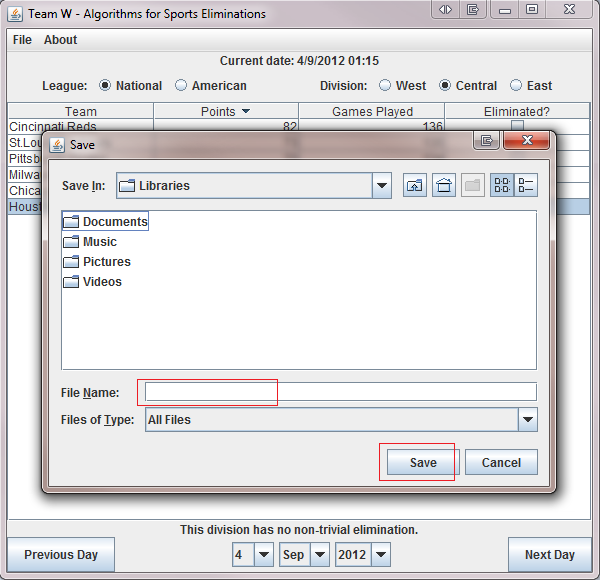
\includegraphics[width=\linewidth,keepaspectratio]{images/userManualDesk8.png}

\newpage

\section{Exporting}

The export functionality with the application allows users to create a PDF file
with chosen days to display. To begin navigate to the file menu and down to
print and if you select ``Add to print'', the program will add the current day
you're on to the printing queue.

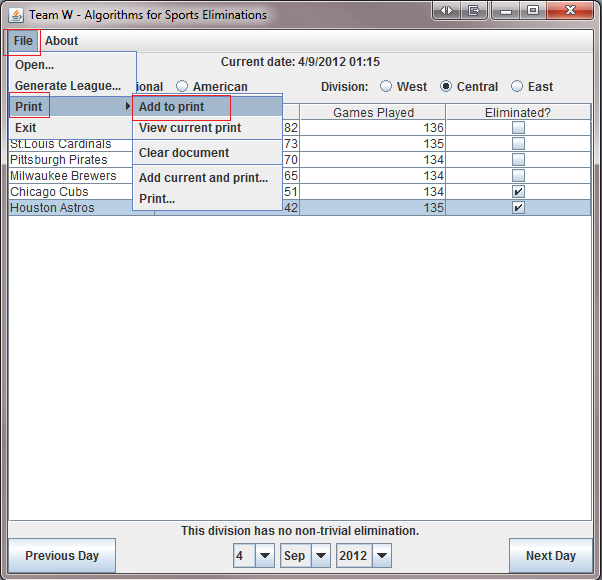
\includegraphics[width=\linewidth,height=\measurepage,keepaspectratio]
{images/userManualDesk9.png}

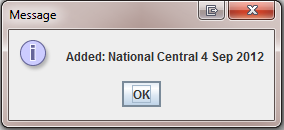
\includegraphics{images/userManualDesk10.png}

\newpage

If you select any number of more dates by navigating however you wish and adding
them one at a time you can then view your print queue and it will show you the
days you wish to export to the PDF.

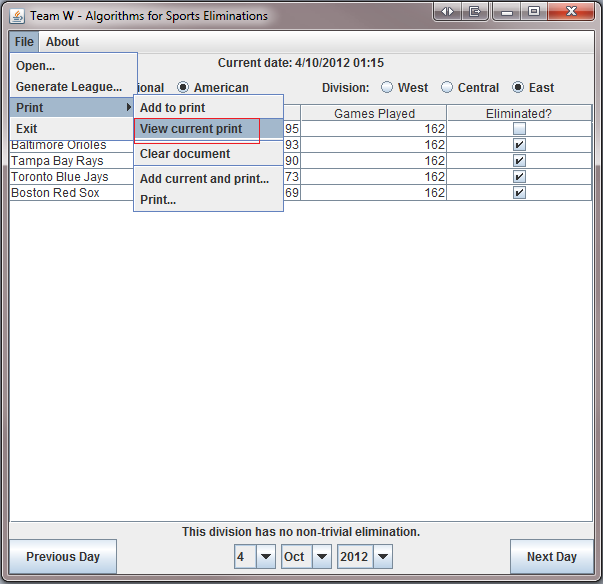
\includegraphics[width=\linewidth,height=\measurepage,keepaspectratio]{images/userManualDesk11.png}

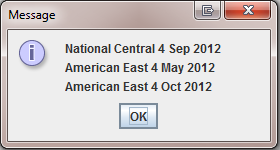
\includegraphics{images/userManualDesk12.png}

\newpage

Finally you can either clear your print queue by selecting ``Clear document'', or
to export your selected results to the PDF simply click ``Print''

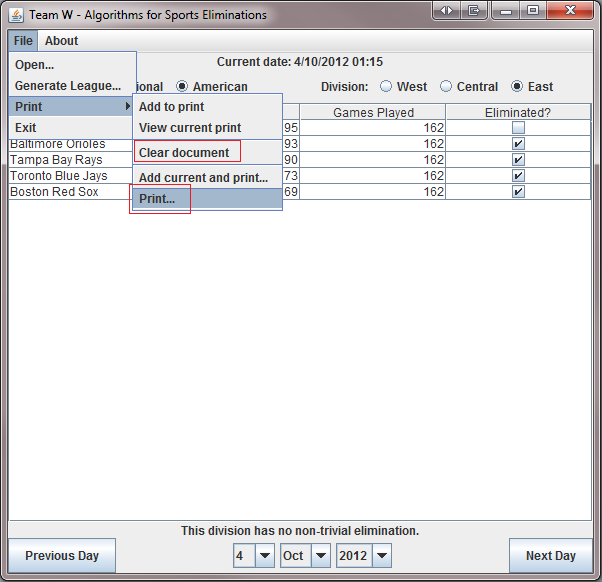
\includegraphics[width=\linewidth,height=\measurepage,keepaspectratio]
{images/userManualDesk13.png}

\newpage

You'll be prompted to select a name for your PDF file in a dialogue box and a
location to save it and then by clicking save your PDF will be compiled ready
for viewing at the specified location.

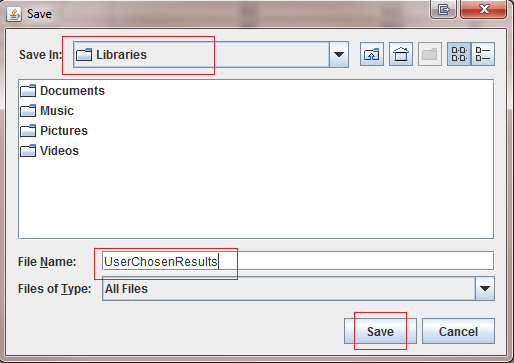
\includegraphics[width=\linewidth,height=\measurepage,keepaspectratio]
{images/userManualDesk14.png}

As we can see below it creates a neatly formatted PDF file of your chosen
results for use outside of the program, showing to others and easily
transferable.

%\includegraphics[width=\linewidth,keepaspectratio]{images/userManualDesk15.png}

\newpage

\section{Web Navigation}

When you first go to the URL specified in the installation chapter you'll be
shown this screen.

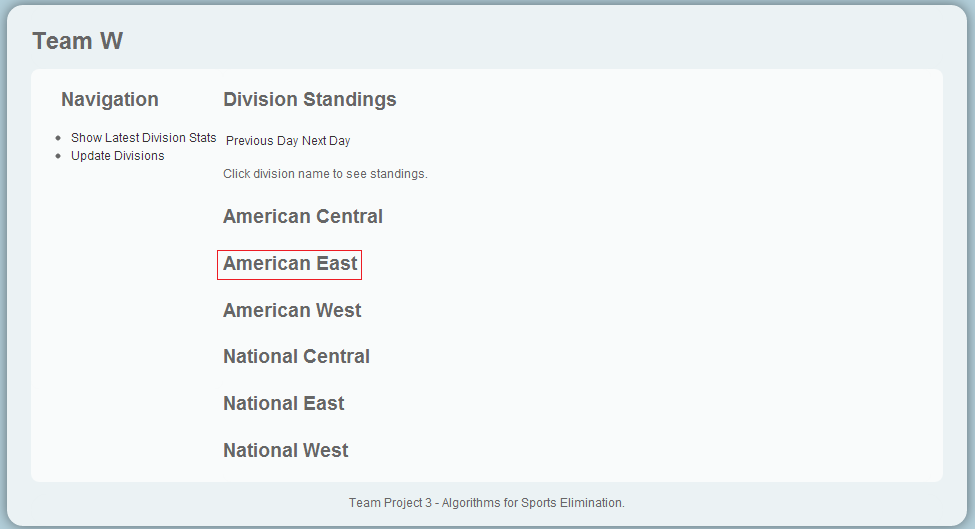
\includegraphics[width=\linewidth,keepaspectratio]{images/userManualWeb1.png}

\newpage

Each of the leagues and divisions are clearly visible and if you click on one of
the emboldened headings the standings will pop out below.

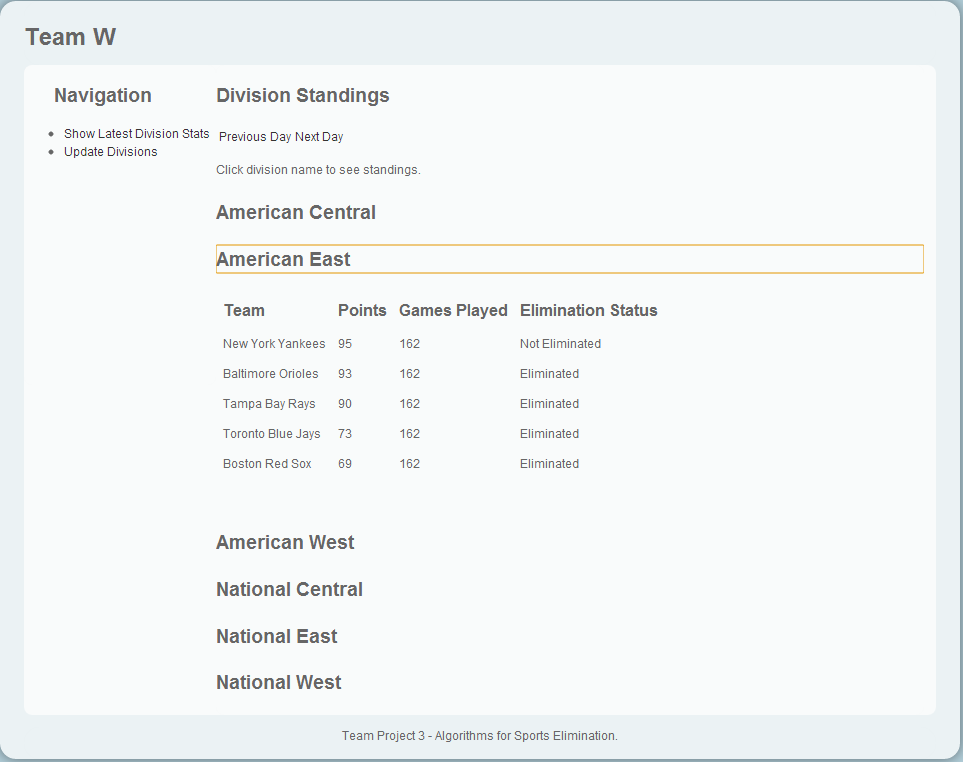
\includegraphics[width=\linewidth,keepaspectratio]{images/userManualWeb2.png}

\newpage

To navigate between different days you can use the previous/next day buttons
above the leagues and divisions.

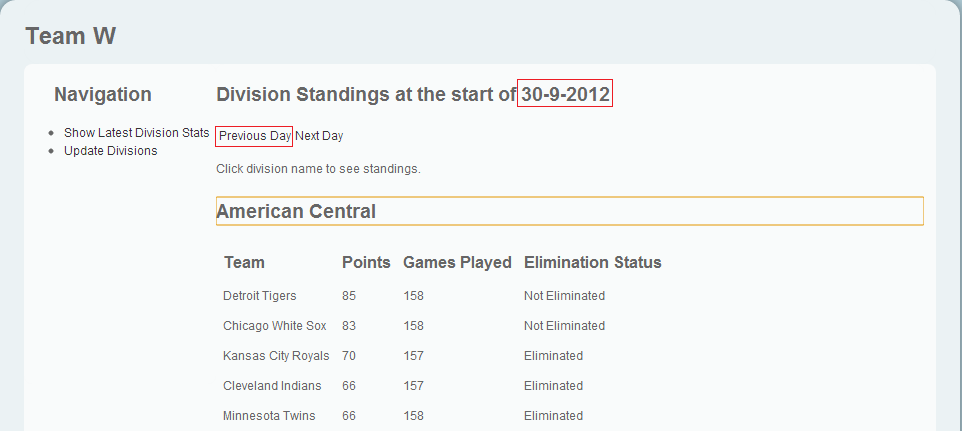
\includegraphics[width=\linewidth,keepaspectratio]{images/userManualWeb3.png}

This method is however very time consuming so instead it would be advised that
you change the date using the URL itself


\includegraphics[width=\linewidth,keepaspectratio]{images/userManualWeb4.png}

Finally if you'd like to jump back to the latest results in a given season you
can click the button in the small side navigation bar.
